\documentclass[notheorems, handout]{beamer}

\usetheme{Warsaw}
\setbeamertemplate{page number in head/foot}[totalframenumber]
\setbeamertemplate{headline}{}
\setbeamertemplate{navigation symbols}{}
\usefonttheme[onlymath]{serif}

\usepackage[utf8]{inputenc}
\usepackage[T2A]{fontenc}
\usepackage[russian]{babel}
\usepackage{graphicx,subcaption,ragged2e}
\usepackage{tikz}
\usepackage{bm}
\usepackage{physics}
\usepackage{amsmath,amsfonts,amssymb}
\usepackage{mathtools}

\newtheorem{theorem}{Теорема}

\title[Нейронные сети для изображений]{Свёрточные нейронные сети для обработки изображений: классификация и сегментация}

\institute[Санкт-Петербургский Государственный Университет]{%
  \small
  Санкт-Петербургский государственный университет\\
  Кафедра статистического моделирования
}
\date{28 октября 2025}
\newcommand{\vect}[1]{\mathbf{#1}}
\newcommand{\matr}[1]{\boldsymbol{#1}}

\begin{document}

\begin{frame}
    \titlepage
\end{frame}

\begin{frame}{Свёрточные нейронные сети (CNN)}
    \begin{itemize}
        \item Класс нейронных сетей, эффективно работающих с изображениями (и другими объектами, в которых важна пространственная связь);
        \item Используют свёртки (свёрточные слои) для извлечения признаков;
        \item Основные применения: классификация, сегментация, детекция объектов.
    \end{itemize}
    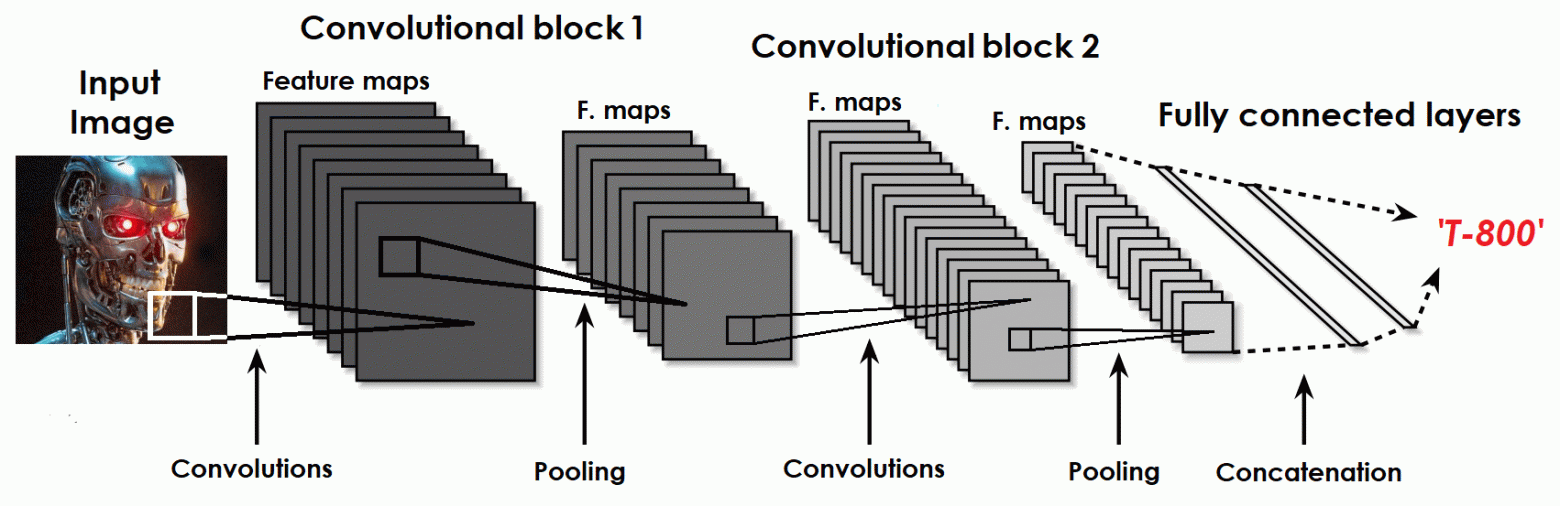
\includegraphics[width=\linewidth]{img/conv_nn.png}
\end{frame}

\begin{frame}{Проблемы обработки изображений полносвязными сетями}
    \begin{itemize}
        \item Изображения содержат пространственную структуру, которую теряют обычные полносвязные сети;
        \item Если изображение имеет высокое разрешение, то полносвязная сеть содержит слишком много параметров;
        \item При небольшом изменении изображения (сдвиг, поворот) входной слой обычной сети полностью меняется, хотя суть осталась прежней.
    \end{itemize}
    \begin{figure}
        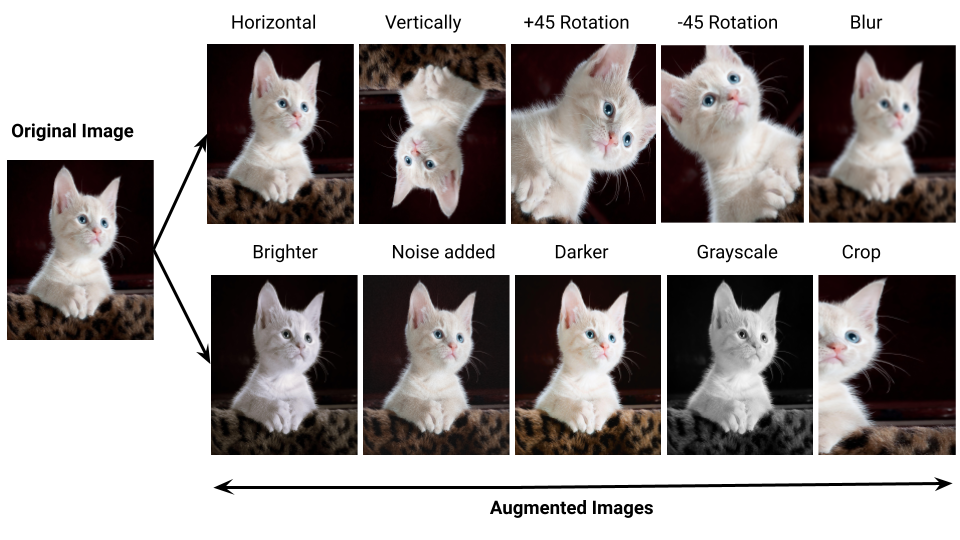
\includegraphics[width=0.7\linewidth]{img/augmentation.png}
    \end{figure}
\end{frame}

\begin{frame}{Основные компоненты CNN}
    \begin{figure}
        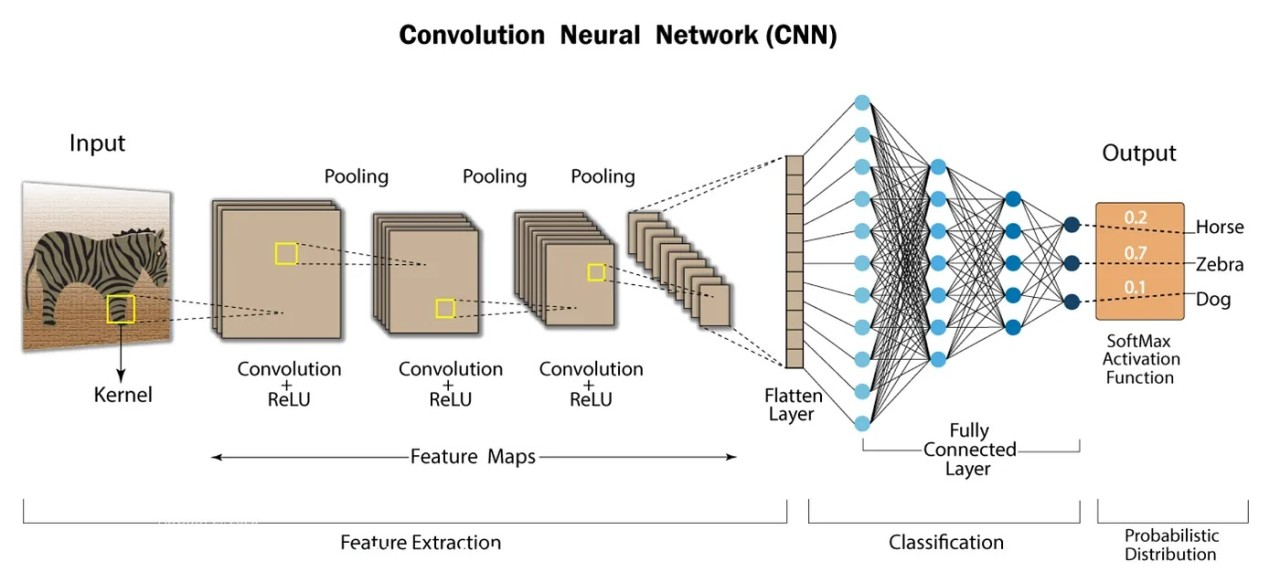
\includegraphics[width=0.8\linewidth]{img/conv_nn_layers.jpeg}    
    \end{figure}

    \begin{itemize}
        \item Свёрточные слои (Conv);
        \item Пулинг (Pooling, часто MaxPooling или AvgPooling);
        \item Нелинейности (ReLU, sigmoid, tanh и т.д.);
        \item Полносвязные слои.
    \end{itemize}

    С помощью свёрточных слоёв и пулинга изображение сводится до вектора размерности $1$, то есть формируется вход для полносвязной сети.
\end{frame}

\begin{frame}{Свёрточная операция}
    \begin{itemize}
        \item Свертка — это скользящее умножение ядра на участок изображения.
        \item Позволяет выделить локальные признаки (границы, текстуры).
    \end{itemize}

    % \[
    %     f _{i, j, c} = b _c + \sum _{p = 1} ^{C _{\text{in}}} \sum _{m = 0} ^{M - 1} \sum _{n = 0} ^{N - 1} W _{c, p, m, n} \,X _{i + m, j + n, p},
    % \]
    % где $W$ --- фильтры размером $M \times N$, $b_k$ --- смещение.

    \begin{figure}
        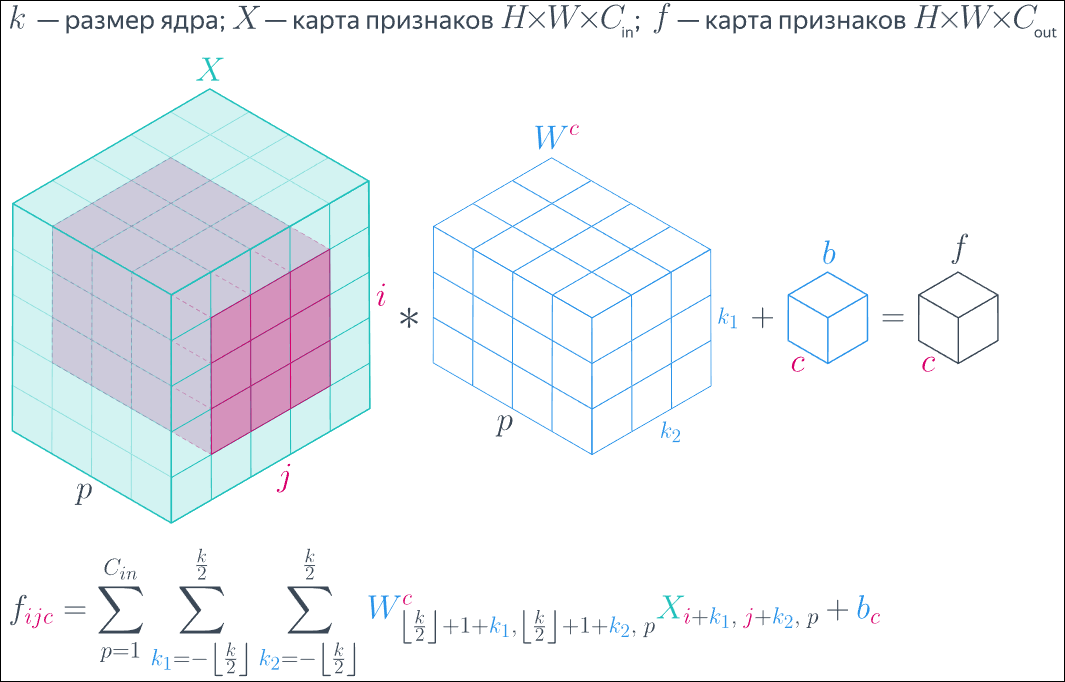
\includegraphics[width=0.9\linewidth]{img/conv_formula.png}
    \end{figure}
\end{frame}

\begin{frame}{Каналы и свёртки}
    \begin{itemize}
        \item Изначально в цветном изображении содержится три канала для каждого цвета;
        \item С каждой свёрткой мы уменьшаем размер изображения, но увеличиваем количество каналов;
    \end{itemize}
    \begin{figure}
        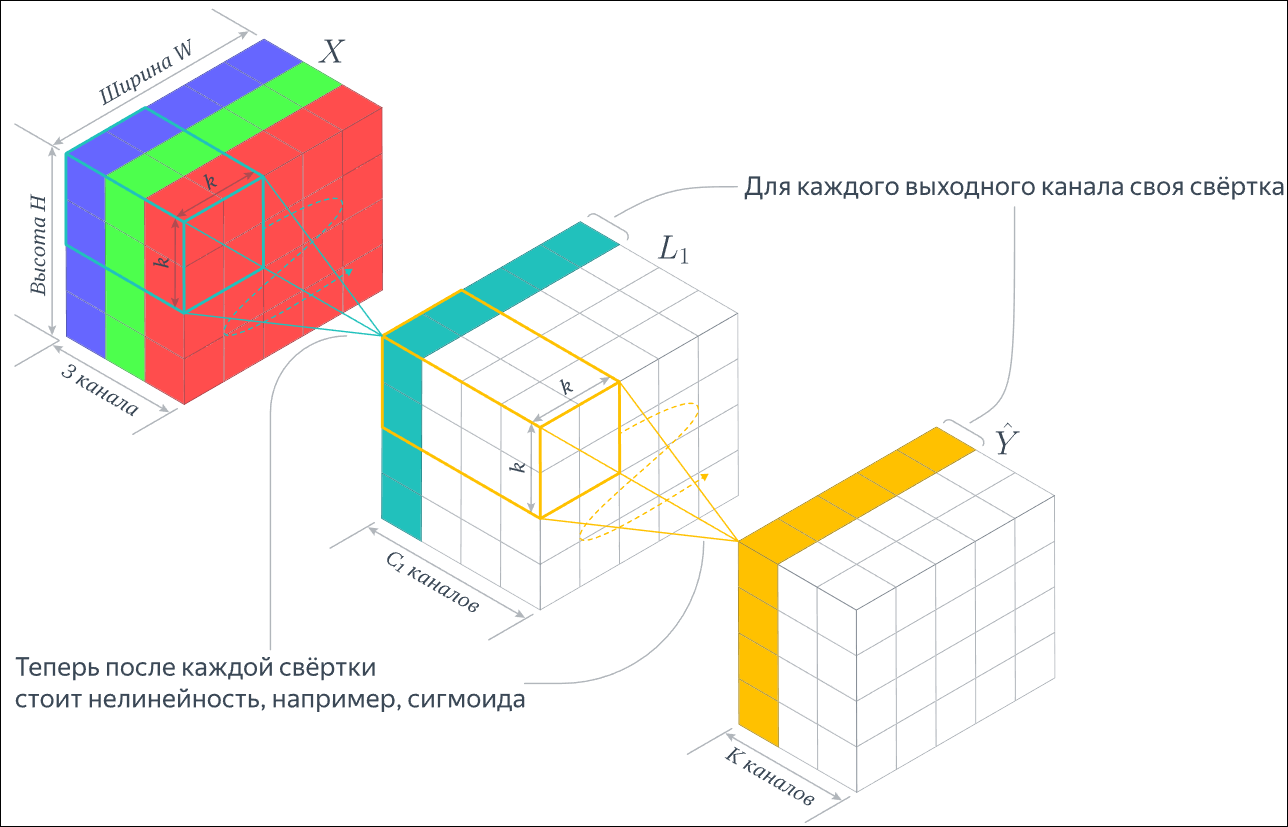
\includegraphics[width=0.8\textwidth]{img/canals.png}
    \end{figure}
\end{frame}

\begin{frame}{Pooling — уменьшение размерности}
    Хотим повысить количество каналов в каждой свёртке, чтобы выделять больше признаков. Проблема: слишком много параметров, решение: уменишить каналы
\begin{itemize}
    \item Max Pooling — берёт максимум из области
    \item Average Pooling — усреднение значений
    \item Снижает вычислительные затраты и переобучение
\end{itemize}
% \includegraphics[width=\linewidth]{placeholder}
\end{frame}

\begin{frame}{ReLU и нормализация}
\begin{itemize}
    \item ReLU: $f(x) = \max(0, x)$ — ускоряет обучение
    \item Batch Normalization стабилизирует распределение активаций
\end{itemize}
% \includegraphics[width=\linewidth]{placeholder}
\end{frame}

\begin{frame}{Задача классификации}
\begin{itemize}
    \item Вход: изображение
    \item Выход: метка класса
    \item Пример: распознавание животных, предметов, сцен
\end{itemize}
% \includegraphics[width=\linewidth]{placeholder}
\end{frame}

\begin{frame}{Популярные архитектуры для классификации}
\begin{itemize}
    \item LeNet (1998)
    \item AlexNet (2012)
    \item VGGNet (2014)
    \item ResNet (2015)
\end{itemize}
% \includegraphics[width=\linewidth]{placeholder}
\end{frame}

\begin{frame}{Пример: ResNet}
\begin{itemize}
    \item Использует остаточные связи (skip-connections)
    \item Позволяет строить очень глубокие сети
    \item Решает проблему затухающего градиента
\end{itemize}
% \includegraphics[width=\linewidth]{placeholder}
\end{frame}

\begin{frame}{Функция потерь и обучение}
\begin{itemize}
    \item Для классификации: Cross-Entropy Loss
    \item Оптимизаторы: SGD, Adam
    \item Используется backpropagation
\end{itemize}
% \includegraphics[width=\linewidth]{placeholder}
\end{frame}

\begin{frame}{Что такое сегментация}
\begin{itemize}
    \item Пиксельная классификация изображения
    \item Цель: выделить объекты на уровне пикселей
    \item Применения: медицина, автономные автомобили, спутниковые снимки
\end{itemize}
% \includegraphics[width=\linewidth]{placeholder}
\end{frame}

\begin{frame}{Виды сегментации}
\begin{itemize}
    \item Семантическая сегментация
    \item Инстанс-сегментация
    \item Паноптическая сегментация
\end{itemize}
% \includegraphics[width=\linewidth]{placeholder}
\end{frame}

\begin{frame}{Архитектуры для сегментации}
\begin{itemize}
    \item U-Net
    \item SegNet
    \item DeepLab
\end{itemize}
% \includegraphics[width=\linewidth]{placeholder}
\end{frame}

\begin{frame}{U-Net}
\begin{itemize}
    \item Симметричная encoder-decoder архитектура
    \item Skip-соединения между слоями
    \item Широко применяется в медицине
\end{itemize}
% \includegraphics[width=\linewidth]{placeholder}
\end{frame}

\begin{frame}{DeepLab}
\begin{itemize}
    \item Использует dilated convolutions
    \item Применяет CRF для уточнения границ объектов
    \item Высокая точность на сложных сценах
\end{itemize}
% \includegraphics[width=\linewidth]{placeholder}
\end{frame}

\begin{frame}{Метрики оценки}
\begin{itemize}
    \item Для классификации: Accuracy, Precision, Recall, F1
    \item Для сегментации: IoU, Dice coefficient
\end{itemize}
% \includegraphics[width=\linewidth]{placeholder}
\end{frame}

\begin{frame}{Применения CNN}
\begin{itemize}
    \item Распознавание лиц, жестов, объектов
    \item Медицинская диагностика
    \item Обработка видео и спутниковых изображений
\end{itemize}
% \includegraphics[width=\linewidth]{placeholder}
\end{frame}

\begin{frame}{Выводы}
\begin{itemize}
    \item CNN — ключевой инструмент компьютерного зрения
    \item Эффективны для классификации и сегментации
    \item Продолжают активно развиваться
\end{itemize}
\end{frame}

\end{document}